%
%     ApJ article: Wreathes of Magnetism in Rapidly Rotating Suns
%     
%     Serious Beginning: June, 2008 (at KITP)
%     Target Completion date : Sep, 2008
%     Submitted :  May 26, 2009
%
%     Benjamin Brown
%
%     Now using AASTex style sheets

%*********************************************************************%
%                                                                     %
%              Introduction section                                   %
%                                                                     %
%*********************************************************************%

\chapter{Global Dynamo that Builds Persistent Wreaths of Magnetism}
%Simulations of Stellar Magnetism and Rotation}
\label{chapter:case D3}

Having explored the coupling of convection and rotation in our
hydrodynamic simulations, it is now time to turn to the question of
possible dynamo action in rapidly rotating suns.  The hydrodynamical
simulations showed us that the shearing flows of differential rotation
generally grow in amplitude with more rapid rotation, possessing rapid
equators and slower poles, while the meridional circulations weaken
and break up into multiple cells in radius and latitude.  More rapid
rotation can also substantially modify the patterns of convection in a
surprising fashion.  With more rapid rotation, localized states begin
to appear in which the convection at low latitudes is modulated in its
strength with longitude.  At the highest rotation rates, the
convection can become confined to active nests which propagate at
distinct rates and persist for long epochs.

Motivated by these discoveries, we turn here to explorations
of the possible dynamo action achieved in solar-type stars rotating at
three and five times the current solar rate.  
%
Magnetism leads to strong feedbacks on the flows,
particularly modifying the differential rotation and its scaling with
overall rotation rate $\Omega_0$.  The magnetic fields which form in these
dynamos have prominent global-scale organization within the convection zone, in contrast to
previous solar dynamo simulations \citep{Brun_et_al_2004, Browning_et_al_2006}.  
Quite strikingly, we find that
coherent global magnetic structures arise naturally in the midst of the
turbulent convection zones.  These wreath-like structures are regions of
strong longitudinal field $B_\phi$ organized loosely into tubes, with fields wandering in
and out of the surrounding convection.  These wreaths of magnetism differ
substantially from the idealized flux tubes supposed in many dynamo
theories, though they may be related to coherent structures
achieved in local simulations of dynamo action in shear flows
\citep{Cline_et_al_2003a, Vasil&Brummell_2008,Vasil&Brummell_2009}.  
Here we explore the nature of magnetic
wreaths realized in our global simulations, and discuss their
temporal behavior.

The contents of Chapters~\ref{chapter:case D3}, \ref{chapter:case D5}
and \ref{chapter:dynamo production} are based on work submitted for
publication as
\cite{Brown_et_al_2009}\footnote{{Brown}, B.~P., {Browning}, M.~K., {Brun}, A.~S., {Miesch}, M.~S., \& {Toomre},
  J., 2009, {Persistent wreathes of magnetism in a rapidly rotating sun}, {\sl \apj},
  ~under review.}
%\footnote{\cite*{Brown_et_al_2009},
%``Persistent Wreaths of Magnetism in a Rapidly Rotating Sun''} 
and are mainly a restatement of that paper under review.  As the
primary author of this paper, I conducted the simulations presented
here, performed the analysis and wrote the text.  My co-authors
provided advice and guidance throughout the process, helping frame the
questions which form the core of the study.  Preliminary versions of
these results have also been presented in
\cite{Brown_AAS_2007a}, \cite{Brown_et_al_2007c},
\cite{Brown_AAS_2009}, and \cite{Brown_SPD_2009}.

%\section{Convection and Dynamos in Rapidly Rotating Systems}

%\section{Dynamos with Persistent Magnetic Wreaths}

We begin by turning to case~D3 whose formulation is shown in
Figure~\ref{fig:energy_D3}.  This dynamo yields fairly persistent
wreaths of magnetism in its two hemispheres, though these structures 
did wax and wane somewhat in strength once established.  Examining the
properties of this dynamo solution helps to provide a perspective for
the greater variations realized in our more rapidly rotating case~D5.

\section{Patterns of Convection in Case~D3}

%\label{sec:steady_dynamo}
The complex and evolving convective structures in our dynamo cases are
substantially similar to the patterns of convection found in our
hydrodynamic simulations.  Our dynamo solution rotating at three times
the solar rate, case~D3, is presented in
Figure~\ref{fig:case_D3_patterns}, along with its hydrodynamic
progenitor, case~H3.  The radial velocities shown near the
top of the simulated domain (Figs.~\ref{fig:case_D3_patterns}$a,e$)
have broad upflows and narrow downflows as a
consequence of the compressible motions.  Near the equator the
convection is aligned largely in the north-south direction, and
these broad fronts sweep through the domain in a prograde fashion.
The strongest downflows penetrate to the bottom of the convection zone;
the weaker flows are partially truncated by the strong zonal flows
of differential rotation.  In the polar regions the convection is more
isotropic and cyclonic.  There the networks of downflow lanes surround upflows
and both propagate in a retrograde fashion.


\begin{figure*}[!t]
%\begin{sidewaysfigure}
  \vskip0.2cm
  \begin{center}
    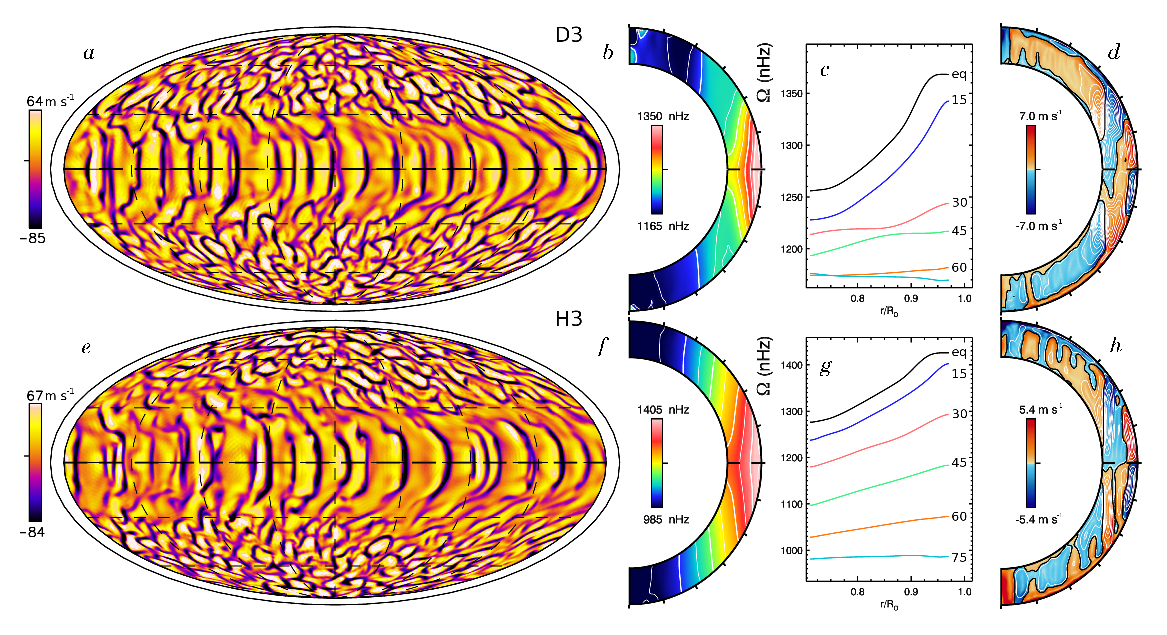
\includegraphics[width=\linewidth]{figs/chapter_5/Figure_1/Figure_1.eps}
  \end{center}
  \caption[Convective structures and mean flows in cases D3 and H3]
	  {Convective structures and mean flows in cases D3 and H3. 
	    $(a)$~Radial velocity $v_r$ in dynamo case D3, shown in global Mollweide projection at
  $0.95R_\odot$, with upflows light and downflows dark.  Poles are at
  top and bottom and the equator is the thick dashed line.  The
  stellar surface at $R_\odot$ is indicated by the thin surrounding
  line.  $(b)$~Profiles of mean angular velocity $\Omega(r,\theta)$,
  accompanied in $(c)$~by radial cuts of $\Omega$ at selected
  latitudes.  A strong differential rotation is established by the
  convection. $(d)$~Profiles of meridional circulation, with sense of
  circulation indicated by color (red counter-clockwise, blue
  clockwise) and streamlines of mass flux overlaid.  
  $(e-h)$~Companion presentation of fields for hydrodynamic progenitor case H3.  The patterns of radial
  velocity are very similar in both cases.  The differential rotation
  is much stronger in the hydrodynamic case and the meridional
  circulations there are somewhat weaker, though their structure
  remains similar.
  \label{fig:case_D3_patterns}}
%\end{sidewaysfigure}
\end{figure*}

\clearpage
The convection establishes a prominent differential rotation profile by
redistributing angular momentum and entropy, building gradients
in latitude of angular velocity and temperature.  
Figures~\ref{fig:case_D3_patterns}$b,f$ show the mean angular velocity
$\Omega(r,\theta)$ for cases D3 and H3, revealing a solar-like
structure with a prograde (fast) equator and retrograde (slow) pole.
This property is also realized for cases D5 and H5 with faster
rotation.  Figures~\ref{fig:case_D3_patterns}$c,g$ present in turn radial
cuts of $\Omega$ at selected latitudes, which are useful as we consider
the angular velocity patterns realized here with faster rotation. 
These $\Omega(r,\theta)$ profiles are averaged in azimuth (longitude)
and time over a period of roughly 200~days. 
Contours of constant angular velocity are aligned nearly
on cylinders, influenced by the Taylor-Proudman theorem.  

As discussed in Chapter~\ref{chapter:introduction}, 
helioseismology has revealed that in the Sun the contours of angular velocity
are aligned almost on radial lines rather than on cylinders.  The tilt
of $\Omega$ contours in the Sun may be due in part to the thermal
structure of the solar tachocline, as first found in the mean-field
models of \cite{Rempel_2005} and then in 3-D simulations  of global-scale
convection by \cite{Miesch_et_al_2006}.  In those computations, it was
realized that introducing a weak latitudinal gradient of entropy at the
base of the convection zone, consistent with a thermal wind balance in
a tachocline of shear, can serve to tilt the $\Omega$ contours
toward a more radial alignment without significantly changing either
the overall $\Omega$ contrast with latitude or the convective
patterns.  We expect similar behavior here, but at present,
observations of rapidly rotating stars only measure differential
rotation at the surface and do not offer constraints on either the
existence of tachoclines in young suns or the nature of their internal
differential rotation profiles.  As such, we have
neglected the possible tachoclines of penetration and shear entirely
in these models and instead adopt the simplification of imposing a
constant radial entropy gradient at the bottom of the convection zone.



The differential rotation achieved is stronger in our hydrodynamic
case~H3 than in our dynamo case~D3.
This can be quantified by measurements of the 
latitudinal angular velocity shear $\Delta \Omega_\mathrm{lat}$.  Here, as in
Chapter~\ref{chapter:convection in G1-G10} %\cite{Brown_et_al_2008}, 
we define $\Delta \Omega_\mathrm{lat}$ as the shear near
the surface between the equator and a high latitude, say $\pm 60^\circ$
\begin{equation}
  \Delta \Omega_\mathrm{lat} = \Omega_\mathrm{eq} - \Omega_{60},
  \label{eq:absolute_contrast}
\end{equation}
and the radial shear $\Delta \Omega_\mathrm{r}$ as the angular
velocity shear between the surface and bottom of the convection zone
near the equator 
\begin{equation}
  \Delta \Omega_\mathrm{r} = \Omega_{0.97R_\odot} - \Omega_{0.72R_\odot}.
  \label{eq:absolute_radial_contrast}
\end{equation}
We further define the relative shear as 
$\Delta \Omega_\mathrm{lat}/\Omega_\mathrm{eq}$.
In both definitions, we average the measurements of $\Delta \Omega$
in the northern and southern hemispheres, as the rotation profile is
often slightly asymmetric about the equator.
Case~H3 achieves an absolute contrast $\Delta \Omega_\mathrm{lat}$ of
2.22~$\mu~\mathrm{rad}\:\mathrm{s}^{-1}$ (352~nHz) and a relative contrast of 0.247.
The strong global-scale magnetic fields realized in the dynamo case~D3
serve to diminish the differential rotation.  As such, this case
achieves an absolute contrast $\Delta \Omega_\mathrm{lat}$ of only 
1.17~$\mu~\mathrm{rad}\:\mathrm{s}^{-1}$ (186~nHz) and a relative contrast of 0.136.
This results from both a slowing of the equatorial rotation rate and
an increase in the rotation rate in the polar regions.  These results
are quoted in Table~\ref{table:delta_omega}, along with related
measurements for our five solar dynamo case~D5 and hydrodynamic cases 
H3~and~H5.  It is interesting to note that in both dynamo cases the
amount of latitudinal and radial shear is almost the same, whereas in
the hydrodynamic simulations the more rapidly rotating case~H5 has
larger angular velocity contrasts than the slower case~H3.


\begin{deluxetable}{lcccc}
    \tabletypesize{\footnotesize}
    \tablecolumns{5}
    \tablewidth{0pt}  % `natural' size 
    \tablecaption{Near-surface $\Delta \Omega$ in Cases at $3$ and $5\thinspace\Omega_\odot$
    \label{table:delta_omega}}
    \tablehead{\colhead{Case}  &  
      \colhead{$\Delta \Omega_\mathrm{lat}$} &
      \colhead{$\Delta \Omega_\mathrm{r}$} &
      \colhead{$\Delta \Omega_\mathrm{lat}/\Omega_\mathrm{eq}$} &
      \colhead{Epoch} 
   }
   \startdata
    D3                        & 1.17 & 0.71 & 0.136 & 6460-6920 \\
    D5$^\text{{avg}}$    & 1.14 & 0.71 & 0.083 & 3500-5700 \\
    D5$^\text{{min}}$    & 0.91 & 0.39 & 0.067 & 3702 \\
    D5$^\text{{max}}$    & 1.43 & 0.98 & 0.102 & 4060 \\
    H3                        & 2.22 & 0.94 & 0.246 &  - \\
    H5                        & 2.77 & 1.31 & 0.192 &  - \\
    % These measurements performed 4/1/2009; see worklog for details
    \enddata
    \tablecomments{Angular velocity shear in units of $\mu
   \mathrm{rad}\: s^{-1}$, with $\Delta \Omega_\mathrm{lat}$ and $\Delta
   \Omega_\mathrm{lat}/\Omega_\mathrm{eq}$ measured near the surface
   ($0.97R_\odot$) and $\Delta \Omega_\mathrm{r}$ measured across the
   full shell at the equator.  For the dynamo cases, these
   measurements are taken over the indicated range of days.  In
   oscillating case~D5, these measurements are averaged over a long
   epoch ({avg}), and are also taken at two instants in time when the
   differential rotation is particularly strong ({max}) and when
   magnetic fields have suppressed this flow ({min}).  The
   hydrodynamic cases are each averaged for roughly 300 days.  Case~D3
   also shows slow variations in $\Delta \Omega_\mathrm{lat}$ over
   periods of about 2000~days.}
\end{deluxetable}



The meridional circulations realized in the dynamo case~D3 are very
similar to those found in its hydrodynamic progenitor (case~H3).  As illustrated
in Figures~1$d, h$, the circulations are multi-celled in radius and
latitude.  The cells are strongly aligned with the rotation axis,
though some flows along the inner and outer boundaries cross the
tangent cylinder and serve to couple the polar regions to the
equatorial convection.  Flows of meridional circulation are slightly
stronger in the dynamo cases than in the purely hydrodynamic cases,
and these flows weaken with more rapid rotation.


\clearpage
\section{Kinetic and Magnetic Energies}
Convection in these rapidly rotating dynamos is responsible for
building the differential rotation and the magnetic fields.  In a
volume averaged sense, the energy contained in the magnetic fields
in case~D3 is about 10\% of the kinetic energy.  About 35\%
of this kinetic energy is contained in the fluctuating convection
(CKE) and about 65\% in the differential rotation (DRKE), whereas
the weaker meridional circulations contain only a small portion
(MCKE).  The magnetic energy is split between the contributions from
fluctuating fields (FME), involving roughly 53\% of the total magnetic
energy, and the energy of the mean toroidal fields (TME) that are
43\% of the total.  The energy contained in the mean poloidal fields
(PME) is only 4\% of the total magnetic energy.  These energies are
quoted in Table~\ref{table:energies} and are defined as
\begin{eqnarray}
  \mathrm{CKE}  &=& \frac{1}{2}\bar{\rho}\Big[\left(v_r - \langle v_r \rangle\right)^2+\left(v_\theta - \langle v_\theta \rangle\right)^2+\nonumber\\
                & & \qquad \left(v_\phi - \langle v_\phi \rangle\right)^2\Big], \\
  \mathrm{DRKE} &=& \frac{1}{2}\bar{\rho}\langle v_\phi \rangle^2, \\
  \mathrm{MCKE} &=& \frac{1}{2}\bar{\rho}\Big(\langle v_r \rangle^2 + \langle v_\theta \rangle^2 \Big),\\
%\end{eqnarray}
%\begin{eqnarray}
  \mathrm{FME}  &=& \frac{1}{8\pi}\Big[\left(B_r - \langle B_r \rangle\right)^2+\left(B_\theta - \langle B_\theta \rangle\right)^2+\nonumber\\
                & & \qquad \left(B_\phi - \langle B_\phi \rangle\right)^2\Big], \\
  \mathrm{TME}  &=& \frac{1}{8\pi}\langle B_\phi \rangle^2, \\
  \mathrm{PME}  &=& \frac{1}{8\pi}\Big(\langle B_r \rangle^2 + \langle B_\theta \rangle^2 \Big).
\end{eqnarray}
where angle brackets denote an average in longitude.

\begin{deluxetable}{lccccccc}
   \tabletypesize{\footnotesize}
    \tablecolumns{7}
    \tablewidth{0pt}  % `natural' size 
    \tablecaption{Energies in Cases at $3$ and $5\thinspace\Omega_\odot$
    \label{table:energies}}
    \tablehead{\colhead{Case}  &  
      \colhead{CKE} &
      \colhead{DRKE} &
      \colhead{MCKE} &
      \colhead{FME} &
      \colhead{TME} &
      \colhead{PME} %&
%      \colhead{ME/KE}
   }
   \startdata
    D3                       & $2.31$ & $4.35$ & $0.010$ &
                               $0.36$ & $0.29$ & $0.029$ \\ %& $0.10$ \\

    D5$^\text{{avg}}$    & $1.85$ & $4.46$ & $0.006$ &
                               $0.55$ & $0.43$ & $0.048$ \\ % & $0.16$ \\

    D5$^\text{{min}}$    & $1.70$ & $2.85$ & $0.005$ &
                               $0.50$ & $0.25$ & $0.062$ \\ %& $0.18$ \\ 

    D5$^\text{{max}}$    & $1.85$ & $7.52$ & $0.007$ &
                               $0.39$ & $0.65$ & $0.042$ \\ % & $0.12$ \\ 

    H3                       & $2.56$ & $22.2\phn\phn$ & $0.012$ &
                                -     &   -    & - \\ % &  - \\

    H5                       & $2.27$ & $34.3\phn\phn$ & $0.008$ &
                                -     &   -    & - \\ % & - \\

    % These measurements performed 4/23/2009; see worklog for details
    \enddata
 \tablecomments{Volume-averaged energy densities relative to the
    rotating coordinate system.  Kinetic energies are shown for
    convection (CKE), differential rotation (DRKE) and meridional
    circulations (MCKE).  Magnetic energies are shown for fluctuating
    magnetic fields (FME), mean toroidal fields (TME) and mean
    poloidal fields (PME).  All energy densities are reported in units of
    $10^{6} \mathrm{erg}\:\mathrm{cm}^{-3}$ and are 
    averaged over 1000 day periods except for time-varying case~D5,
    where intervals are as in Table~\ref{table:delta_omega}.}
\end{deluxetable}

% Case D3
%average drke:      4351087.1 ($  65.182\% $) 
%average mcke:        10351.298 ($   0.155\% $) 
%average  cke:      2310531.7 ($  34.662 \% $) 
%average  me:        673295.33 ($  10.156\% $) 
%average tme:        286349.77 ($   4.317\% $)  ($  42.617\% $) 
%average pme:         28575.044 ($   0.435\% $)  ($   4.183\% $) 
%average fme:        358370.52 ($   5.404 \% $)  ($  53.199 \% $) 

%D5 min
%IDL> print, f[(find_value(4060, t-t[0])),*]
%  4.56427e+06      ; total KE
%  2.85383e+06
%      4658.62
%  1.70578e+06
%      818788.      ; total ME
%      253718.
%       62447.3
%      502623.

% D5 max
%IDL> print, f[(find_value(3702, t-t[0])),*]
%  9.38107e+06      ; total KE
%  7.52216e+06
%      7361.79
%  1.85155e+06
%  1.08589e+06      ; total ME
%      648911.
%       42301.7
%      394681.

% D5 avg
%average drke:        4461817.5 ($        71.521201\% $) 
%average mcke:           6401.5652 ($      0.092478704\% $) 
%average  cke:        1845690.8 ($        28.386332 \% $) 
%average   me:        1034037.5 ($        13.693244\% $) 
%average  tme:         432782.37 ($        4.9087451\% $)  ($        38.032929\% $) 
%average  pme:          47827.404 ($       0.70125941 \% $)  ($        4.8328900\% $) 
%average  fme:         553427.62 ($        8.0832380\% $)  ($        57.134171\% $) 

% case H3
% average drke:        22208338. ($  89.613\% $) 
% average mcke:           12015.076 ($   0.048\% $) 
% average  cke:         2562315.4 ($  10.339 \% $) 

% case H5
% average drke:        34291361. ($  93.778\% $) 
% average mcke:            7614.8481 ($   0.021\% $) 
% average  cke:         2267879.9 ($   6.201 \% $) 



These results are in contrast to our previous simulations of the solar
dynamo, where the mean fields contained only about 2\% of the magnetic
energy and the fluctuating fields contained nearly 98\%
\citep{Brun_et_al_2004}.  In simulations of the solar dynamo that
included a stable tachocline at the base of the convection zone
\citep{Browning_et_al_2006}, the energy of the mean fields in the
tachocline can exceed the energy of the fluctuating fields there 
by about a factor of three, though 
the fluctuating fields still dominate the magnetic
energy budget within the convection zone itself.  Simulations of dynamo
activity in the convecting cores of A-type stars
\citep{Brun_et_al_2005} achieved similar results.  There in the
stable radiative zone the energies of the mean fields were able to
exceed the energy contained in the fluctuating fields, but in the
convecting core the fluctuating fields contained roughly 95\% of the
magnetic energy.  Simulations of dynamo action in fully-convective
M-stars do however show high levels of magnetic energy in the mean
fields \citep{Browning_2008}. In those simulations the fluctuating
fields still contain much of the magnetic energy,
but the mean toroidal fields possess about 18\% of the total
throughout most of the stellar interior. 
In our rapidly rotating suns, the mean fields
comprise a significant portion of the magnetic energy in the
convection zone and are as important as the fluctuating fields.

Convection is similarly strong in all four rapidly rotating cases, and
CKE is similar in magnitude.  The differential rotation in the dynamo
cases is much weaker than in the hydrodynamic progenitors and DRKE has decreased by
about a factor of five.  The magnetic fields and differential rotation
in case~D5 change in time, but the average energy contained in DRKE is
nearly the same in both dynamo cases despite their very different
rotation rates.  This is in striking contrast to the behavior of the
hydrodynamic cases, where DRKE is much larger in the more rapidly
rotating case~H5 than in case~H3.  Meridional circulations are
comparably weak in all cases. 

The amount of energy contained in the magnetic fields is different in
these two dynamo cases, with energies generally stronger in case~D5
than in case~D3. In an average sense, all three magnetic energies are
about 1.5 times greater in case~D5 than in case~D3.  Case~D5 shows
substantial time variation, and at periods either FME or TME can become
quite similar to those values realized in case~D3.  Meanwhile, PME is always
stronger in D5 than in D3.


\section{Wreaths of Magnetism}
\label{sec:wreaths}

These dynamos produce striking magnetic structures in the midst of
their turbulent convection zones.  The magnetic field is organized
into large banded, wreath-like structures positioned near the equator
and spanning the depth of the convection zone.  These wreaths are shown
at two depths in the convection zone in Figure~\ref{fig:case_D3_many_depths}.   
The dominant component of the magnetic wreaths is the strong longitudinal
field $B_\phi$, with each wreath possessing its own polarity.  The average
strength of the longitudinal field at mid-convection zone is $\pm 7$~kG 
and peak field strengths there reach roughly $\pm 26$~kG.  
Threaded throughout the wreaths are weaker radial and latitudinal magnetic
fields, which connect the two structures across the equator and also
to the high-latitude regions.  

These wreaths of magnetism survive despite being embedded in vigorous
convective upflows and downflows.  The
convective flows leave their imprint on the magnetic structures,  
with individual downflow lanes entraining the
magnetic field, advecting it away, and stretching it into $B_r$
while leaving regions of locally reduced $B_\phi$. The slower upflows
carry stronger $B_\phi$ up from the depths.  Where the magnetism is
particularly strong the convective flows are disrupted.
Meanwhile, where the convective flows are strongest, the longitudinal
magnetic field is weakened and appears to 
vanish.  In  reality, the magnetic wreaths here are
diving deeper below the mid-convection zone, apparently pumped
down by the pummeling action of the strong downflows.  

\begin{figure*}
  \begin{center}
    \includegraphics[width=\linewidth]{figs/chapter_5/Figure_2/Figure_2.eps}
  \end{center}
  \caption[Magnetic and convective structures in case D3 at two depths]
	  {Magnetic wreaths and convective flows sampled at the same instant in
    case D3.   $(a)$~Longitudinal magnetic field $B_\phi$ near the top of the shell
    ($0.95R_\sol$) and ($b$)~at mid-depth ($0.85R_\sol$).  Strong
    flux structures with opposite polarity lie above and below the equator
    and span the convection zone.  ($c,d$)~Weaker radial magnetic
    field $B_r$ permeates and encircles each wreath. ($e,f$)~Strong convective upflows
    and downflows shown by $V_r$ pass through and around
    the wreaths.  The regions of strong magnetism tend to disrupt the
    convective flows while the strongest downflows serve to
    pump the wreaths to greater depths.
  \label{fig:case_D3_many_depths}}
\end{figure*}

\begin{figure*}
  \begin{center}
    \includegraphics[width=0.85\linewidth]{figs/chapter_5/Figure_3/Figure_3.eps}
  \end{center}
  \caption[Field line visualization of magnetic wreaths in case~D3]
	  {Field line visualization of magnetic wreaths in case~D3.
    $(a)$~Snapshot of two wreaths in full volume at same instant
    as in Fig.~\ref{fig:case_D3_many_depths}.  Lines
    trace the magnetic fields, color denoting the amplitude and
    polarity of the longitudinal field $B_\phi$ (red, positive;
    blue, negative).  Magnetic field threads in and out of the wreaths,
    connecting the two opposite polarity structures across the equator
    (i.e., region A) and to the polar  regions where the magnetic field
    is wound up by the cyclonic convection.
    $(b)$~Same snapshot showing south polar region.  
    $(c)$~Zoom in on region A showing the complex interconnections
    across the equator between the two wreaths and to high
    latitudes.  Convective flows create the distinctive waviness
    visible in all three images.
  \label{fig:case_D3_field_lines}}
\end{figure*}



The deep structure of these wreaths is revealed by field line
tracings throughout the volume, shown in
Figure~\ref{fig:case_D3_field_lines} for the same instant in time.
The wreaths are topologically leaky structures, with magnetic field
lines threading in and out of the surrounding convection.  The
wreaths are connected to the high-latitude (polar) convection, and on
the poleward edges they show substantial winding from the highly
vortical convection found there.  This occurs in both the northern and
southern hemispheres, as shown in two views at the same instant
(north, Fig.~\ref{fig:case_D3_field_lines}$a$ and south,
Fig.~\ref{fig:case_D3_field_lines}$b$).  It is here that the
global-scale poloidal field is being regenerated by the coupling of
fluctuating velocities and fluctuating fields. Magnetic fields cross the
equator, tying the two wreaths together at many locations
(Fig.~\ref{fig:case_D3_field_lines}$c$).  The strongest convective
downflows leave their imprint on the wreaths as regions where the
field lines are dragged down deeper into the convection zone, yielding
a wavy appearance to the wreaths as a whole.


\section{Wreaths Persist for Long Epochs}
The wreaths of magnetism built in case~D3 persist for
long periods of time, with little change in strength and no reversals
in global-scale polarity for as long as we have pursued
these calculations.  The long-term stability of the wreaths realized
by the dynamo of case~D3 is shown in Figure~\ref{fig:case_D3_time_evolution}.
Here the azimuthally-averaged longitudinal field $\langle B_\phi \rangle$
and colatitudinal field $\langle B_\theta \rangle$ are shown at
mid-convection zone at a point after the dynamo has equilibrated and
for a period of roughly 5000~days (i.e.,~several ohmic diffusion times).  
During this interval there is little
change in either the amplitude or structure of the mean fields.  This
is despite the short overturn times of the convection (10-30
days) or the rotation period of the star ($\sim 9$~days).  The ohmic
diffusion time at mid-convection zone is approximately 1300 days.

Though the mean (global-scale) fields are roughly steady in nature
(Figs.~\ref{fig:case_D3_time_evolution}$a,b$), the magnetic
field interacts strongly with the convection on smaller scales. 
Several samples of longitudinal field $B_\phi$ are shown in full Mollweide projection at
mid-convection zone (Fig.~\ref{fig:case_D3_time_evolution}$c$).  
The magnetic fields are clearly reacting on short time scales to the
convection but the wreaths maintain their coherence.  

%\begin{sidewaysfigure}
\begin{figure*}[!t]
  \vskip0.2cm
  \begin{center}
    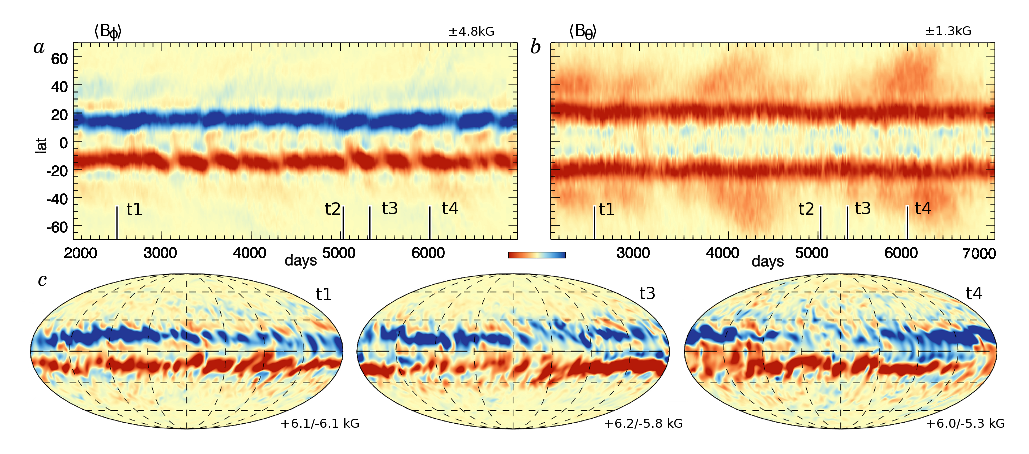
\includegraphics[width=\linewidth]{figs/chapter_5/Figure_4/Figure_4.eps}
  \end{center}
  \caption[Persistent wreaths of magnetism in case~D3]
          {Persistent wreaths of magnetism in case~D3.  
  $(a)$~Time-latitude plots of
  azimuthally-averaged longitudinal field $\langle B_\phi \rangle$ 
  at mid-convection zone ($0.85R_\sol$) in a view spanning latitudes from
  $\pm 70^\circ$, with scaling values
  indicated.  The two wreaths of opposite polarity persist for more
  than 4000 days. $(b)$~Mean colatitudinal magnetic field 
  $\langle B_\theta \rangle$ at
  mid-convection zone over same interval.  $(c)$~Snapshots of $B_\phi$
  in Mollweide projection at mid-convection zone, shown for three
  times indicated in $a,b$.  The wreaths maintain constant polarity
  over long time intervals, but still show variation as they interact
  with the convection.  Time t2 corresponds to the snapshot in 
  Fig.~\ref{fig:case_D3_many_depths}$b$.
  \label{fig:case_D3_time_evolution}}
%\end{sidewaysfigure}
\end{figure*}


There are also some small but repeated variations in the global-scale magnetic fields.
Visible in Figure~\ref{fig:case_D3_time_evolution}$b$ are
events where propagating structures of $\langle B_\theta \rangle$ reach toward
higher latitudes over periods of about 1000~days (i.e., from day 3700
to day 4500 and from day 5600 to day 6400).  These are accompanied by
slight variations in the volume-averaged magnetic energy densities and
the comparable kinetic energy of the differential rotation.
These variations are also visible in the differential rotation itself,
as shown in Figure~\ref{fig:case_D3_DR}.  The differential rotation
is fairly stable, though some time variation is visible at high
latitudes.  This is better revealed (Fig.~\ref{fig:case_D3_DR}$b$)
by subtracting the time-averaged profile of $\Omega$ at each
latitude, revealing the temporal variations about this mean.   
In the polar regions above $\pm 40^\circ$ latitude, speedup features
move poleward over 500 day periods.  These features
track similar structures visible in the mean magnetic fields
(Fig.~\ref{fig:case_D3_time_evolution}$b$).   

\begin{figure}
  %\vspace{1cm}
  \begin{center}
    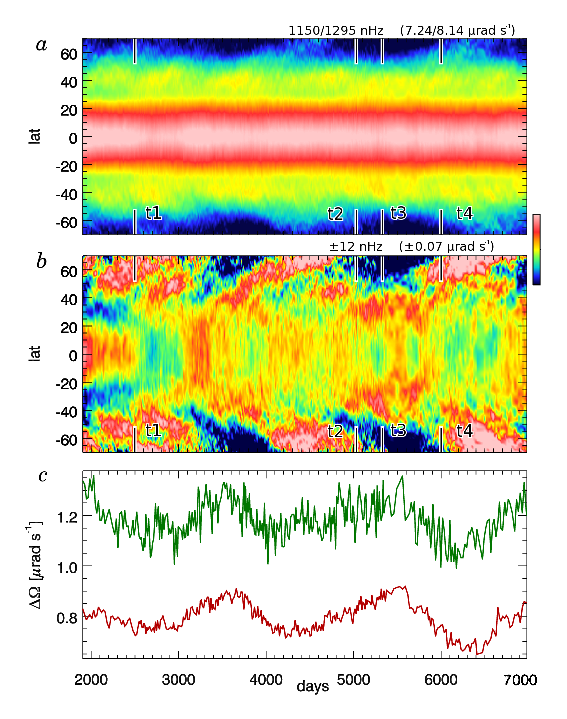
\includegraphics[width=0.8\linewidth]{figs/chapter_5/Figure_5/Figure_5.eps}
  \end{center}
  \caption[Temporal variations of differential rotation in case~D3]
	  {Temporal variations of differential rotation in case~D3.  $(a)$~Angular velocity
  $\Omega$ at mid-convection zone ($0.85R_\sol$), with ranges in both nHz
  and $\mu\mathrm{rad}\:\mathrm{s}^{-1}$.  The equator is
  fast while the poles rotate more slowly.  
  $(b)$~Temporal variations are emphasized by subtracting the
  time-averaged profile of $\Omega(r,\theta)$, revealing
  speedup structures at high latitudes and pulses of fast and slow
  motion near the equator.  These bands have average amplitudes of
  $\pm 20\:\mathrm{m}\:\mathrm{s}^{-1}$  and peak amplitudes of about
  $\pm 60\:\mathrm{m}\:\mathrm{s}^{-1}$.  $(c)$~Angular velocity
  shear $\Delta \Omega_\mathrm{lat}$ (eq.~\ref{eq:absolute_contrast}) near the
  surface (upper~curve, green) and at mid-convection zone (lower, red).
  \label{fig:case_D3_DR}
  }
\end{figure}


These evolving structures of magnetism and faster and slower
differential rotation appear to be the
first indications of behavior where the mean fields themselves begin to
wax and wane substantially in strength. As the magnetic Reynolds number is increased,
this time varying behavior becomes more prominent and can even result
in organized changes in the global-scale polarity.  Such behavior is
evident in our case~D5.



\section{Conclusions}

The ability for a dynamo to build wreaths of strong magnetic fields in the bulk of
the convection zone has largely been a surprise, for it had generally
been supposed that turbulent convection would disrupt such magnetic
structures.  To avoid these difficulties, many solar and stellar
dynamo theories shift the burden of magnetic storage, amplification
and organization to a tachocline of shear and penetration at the base
of the convection zone where motions are more quiescent.  In contrast,
our simulations of rapidly rotating stars are able to achieve
sustained global-scale dynamo action within the convection zone
itself, with the magnetic structures both being built and able to survive
while embedded deep within the turbulence.  
These dynamos are able to circumvent the Parker instability by means
of turbulent Reynolds and Maxwell stresses that contribute to the
mechanical force balance and prevent the wreaths from buoyantly
escaping the convection zone.  
This striking behavior may be enabled by the stars rotating three to
five times faster than the current Sun, which yields a strong
differential rotation that is a key element in the dynamo behavior.  
It is quite interesting that in our dynamo cases the angular velocity
contrast in latitude and radius is almost constant at differing
rotation rates, whereas our hydrodynamic cases tend to have increasing
$\Delta \Omega$ with more rapid rotation $\Omega_0$.
  
As we have seen in this chapter, we have achieved some dynamo states
that are persistent. Others flip the sense of their magnetic fields.  
In our case~D3 the global-scale fields have small vacillations in
their amplitudes, but the magnetic 
wreaths retain their identities for many thousands of days.  This
represents hundreds of rotation periods and several magnetic diffusion
times, indicating that the dynamo has achieved a persistent
equilibrium.  As we will see next in Chapter~\ref{chapter:case D5},
increasing the rotation rate yields more complex time
dependence.  
